\documentclass{article}
\usepackage[spanish]{babel}
\usepackage[utf8]{inputenc}
\usepackage{mathtools}
\usepackage{graphicx}
\usepackage[usenames]{color}
\usepackage{hyperref}
\usepackage{parskip}

\title{\Huge Aplicaciones de guía para personas con discapacidad visual}
\author{Clara y Belén}

\setlength{\parskip}{12pt}
\setlength{\parindent}{12pt}

\begin{document}
	
	
	\begin{titlepage}
		\maketitle
		\thispagestyle{empty}
	\end{titlepage}
	
	%ABSTRACT
	\begin{abstract}
	    En los últimos años ha aumentado la concienciación acerca de la importancia de desarrollar tecnologías accesibles e inclusivas, de modo que, concretamente, cada vez son más las aplicaciones que tratan de reducir las limitaciones que antes las convertían en inalcanzables para personas con discapacidad visual.
	    
	    Entre ellas encontramos todo tipo de categorías: redes sociales, entretenimiento, lectura, identificación de colores y objetos, etc. 
	    
	    Nosotras haremos un pequeño estudio sobre qué apliaciones accesibles ya existen en el campo de la navegación, bien sea por interiores o exteriores, y cómo funcionan.
	
	\end{abstract}
	
	
	\section{Aplicaciones de guía para personas con discapacidad visual}
	
	%PRIMERA APP
	\subsection{Google Maps}
		El pasado 10 de Octubre de 2019, en el ``World Sight Day'', Google dió a conocer la última actualización de la famosa aplicación \textit{Google Maps}\footnote{\url{https://blog.google/products/maps/better-maps-for-people-with-vision-impairments/}}. Esta incluiría una nueva característica desarrollada desde cero por y para personas con discapacidad visual que convertiría a la misma en una app accesible.
		
		El proyecto consiste en la implementación de una nueva funcionalidad, que facilita la posibilidad de recibir instrucciones de voz más detalladas y nuevos tipos de anuncios verbales muy útiles para las rutas de a pie. Algunas de las nuevas instrucciones incluídas son: informar de manera proactiva que estás en la ruta correcta, la distancia hasta el próximo giro, la dirección en la que estás caminando, avisos para cruzar con precaución si te aproximas a una gran intersección, notificaciones en caso de ser redirigido por causa de haber abandonado accidentalmente la ruta correcta, etc. De esta manera, la aplicación pretende brindar de independencia a las personas que padecen ceguera tratando de que se sientan cómodas y seguras a la hora de explorar lugares nuevos y desconocidos. La guía de voz detallada para la navegación está actualmente en desarrollo, estando ya disponible en inglés en los Estados Unidos y en japonés en Japón. Su soporte para otros idiomas y países sigue en camino.
		
		En cuanto a la navegación por interiores, \textit{Google Maps}\footnote{\url{https://www.google.es/intl/es/maps/about/partners/indoormaps/}} con su actualización \textit{6.0} incorporó los primeros planos de ciertos edificios, entre los cuales destacan aeropuertos, centros comerciales, estadios y puntos de transporte público.
		
		Gracias a esta nueva versión, \textit{Google Maps} ayuda a determinar dónde estás, en qué planta y hacia dónde ir. Para ello, basta con hacer zoom sobre un edificio cuyo plano esté disponible en la app, y éste aparecerá automáticamente y completamente detallado. En la figura \ref{fig:ejemplo}, por ejemplo, vemos un ejemplo del famoso Madison Square Garden de Nueva York. 
		
		 \begin{figure}[t]
			\centering
			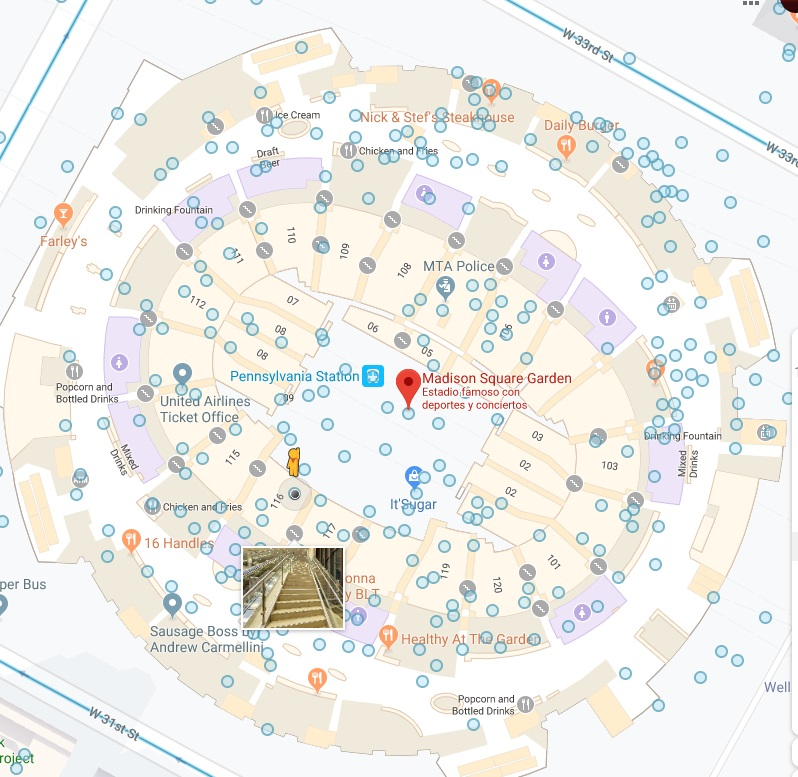
\includegraphics[width=0.6\textwidth]{MadSq2}
			\caption{Plano de un edificio proporcionado por Google Maps.}
			\label{fig:ejemplo}
		\end{figure}
		
		 \begin{figure}[t]
			\centering
			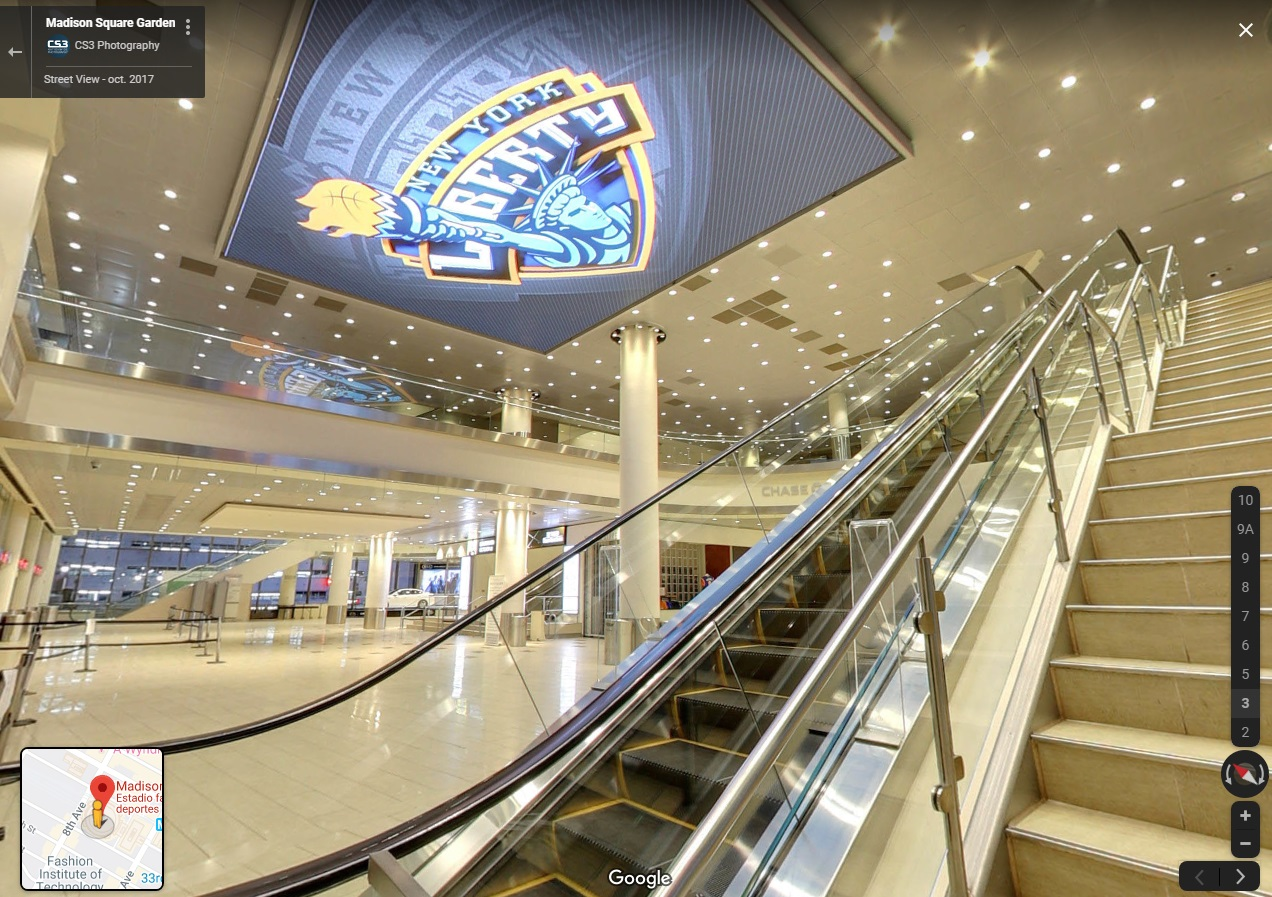
\includegraphics[width=0.6\textwidth]{MadSq3}
			\caption{Vista del interior del Madison Square Garden. }
			\label{fig:ejemplo2}
		\end{figure}
	    
		En el plano podrás localizar dónde están los baños, escaleras, ascensores, entradas y salidas, etc. los cuales aparecen representados mediante los iconos globalmente aceptados (ver figura \ref{fig:ejemplo}). También aparecen detallados los distintos establecimientos que se localizan en el edificio e incluye la posibilidad de hacer ciertas búsquedas, tanto generales (de cafeterías, librerías, tiendas, restaurantes...) como concretas (Starbucks, McDonald...) (ver figura \ref{fig:ejemplo3}). Otra funcionalidad que no falta en la versión de interiores es la posibilidad de señalar un destino y recibir indicaciones sobre cómo llegar a el. Para ello, aparece el habitual punto azul que te acompaña e indica tu posición, actualizando el plano con cada movimiento que lleves a cabo (incluidos cambios de una planta a otra) (ver figura \ref{fig:ejemplo3}).
		
		 \begin{figure}[t]
			\centering
			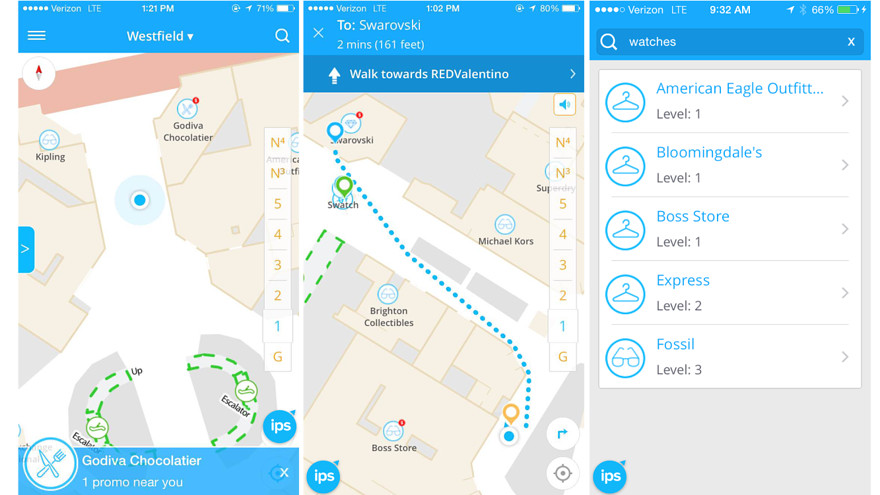
\includegraphics[width=0.6\textwidth]{GMapsInd}
			\caption{Ejemplo de navegación y búsqueda en Google Maps Indoors. }
			\label{fig:ejemplo3}
		\end{figure}
		Esta aplicación es un proyecto colaborativo y por ende, desde la web es posible actualizar y subir nuevos planos. Está disponible tanto para ordenador como plataformas Android e iOS.
	
		Pese al gran avance que supone en la navegación por interiores, cuenta con ciertas desventajas. El posicionamiento, al contrario que en exteriores, no es muy preciso y las búsquedas que puedes realizar son limitadas, no pudiendo, por ejemplo, preguntar por la ubicación de los baños. Pero, sobre todo tiene el inconveniente de que no es una tecnología accesible. \textit{Google Maps Indoors}\footnote{\url{https://www.youtube.com/watch?v=cPsTWj_O3Qs}} es una aplicación completamente visual que no cuenta con soporte auditivo por lo que descarta completamente a usuarios invidentes.
	
		
	%SEGUNDA APP
	\subsection{BlindSquare}
	    Es una de las aplicaciones de navegación más populares, su uso se extiende en más de 130 países y está habilitada en 25 idiomas, entre los cuales se incluye el español. Esta aplicación, desarrollada para iOs y diseñada para personas con discapacidad visual, proporciona una guía completa, de origen a destino, tanto en exteriores como en interiores. Además, describe el entorno y anuncia posibles puntos de interés para el usuario (como pueden ser los lugares considerados populares o aquellos visitados frecuentemente). Su principal característica es que permite interactuar mediante voz gracias al controlador de música de Apple. 
	
	    \textit{BlindSquare}\footnote{\url{https://www.blindsquare.com}} determina tu posición mediante localización \textit{GPS} y, a partir de ahí, puede darte información sobre las proximidades utilizando \textit{Foursquare} y \textit{OpenStreetMap}, de este modo, es capaz tanto de guiarte a un cierto destino como de notificarte qué establecimientos hay en tu radio: restaurantes a 200m, parques más cercanos, farmacias...
	
	    Con el fin de agilizar el uso de la app y que por tanto, esta sea cómoda y rentable para los usuarios finales, incluye: accesos directos a funciones mediante gestos, como sacudir el móvil para que nos diga la ubicación actual y puntos cercanos; y, la posibilidad de establecer filtros para recibir únicamente información deseada. Filtrar por restaurantes para no tener notificaciones sobre estaciones de tren o librerías.
	
	    En cuanto a la localización por interiores, \textit{BlindSquare}\footnote{\url{https://www.youtube.com/watch?v=9jH-Bdjmgb4}} emplea \textit{beacons} y ¿¿VPS?? para solventar el problema del posicionamiento. Por lo demás, incluye las mismas posibilidades y funcionalidades que la navegación por exteriores, con la única limitación de que el edificio debe estar provisto de dichos sistemas de posicionamiento.
	
	    Puntos fuertes de esta aplicación:
	    \begin{itemize}
		    \item Da información sobre los metros que quedan hasta llegar a un determinado objetivo. Resulta útil porque si van disminuyendo sabes que vas por el camino adecuado.
		    \item Utiliza indicaciones reloj: a las 10, a las 3,...
		    \item Te avisa de las intersecciones. 
		    \item Cuando te da una nueva indicación y la superas salta el sonido asociado a correto o check. Así, puedes seguir sin preocuparte. Si por el contrario te equivocas te salta un sonido en consecuencia.
		    \item Se pueden añadir ubicaciones en una lista de lugares marcados.
		    \item Puedes ir girando con el móvil y te va indicando lo que tienes enfrente. 
		    \item También tiene opción de simulación, que permite prepararse un camino antes de ir.
		    \item Te permite ser más autónomo y descubrir nuevos sitios.
		    \item A la hora de desplazarte te indica las opciones por adelantado. Bus, metro, etc. para espacios exteriores o, escaleras, ascensor, escaleras mecánicas, etc. en el caso de interiores.
		    \item Permite llevar las manos libres.
		    \item Incluye un lector de códigos QR, es más cómodo porque puede dar más información que la línea braille.
	    \end{itemize}

	    Entre sus puntos negativos: cuesta 40 libras.
	
	\subsection{Nearby Explorer}
	    \textit{Nearby Explorer}\footnote{\url{https://play.google.com/store/apps/details?id=org.aph.nearbyonline&hl=es}} es otra de las aplicaciones que encuadramos en el campo de la navegación accesible por interiores y exteriores. Está habilitada tanto para Android como para iOs y su descarga se encuentra disponible en el \textit{App Store} de manera gratuita. 
	
	    La guía por exteriores se basa en la misma idea que \textit{BlindSquare} y por ende, funciona de manera similar. Entre sus características destacan: la posibilidad de ejecutar ciertas acciones poniendo el móvil en distintas posiciones, como por ejemplo, inclinarlo verticalmente para que funcione como una brújula; y, la capacidad de filtrar la información de modo que ésta se adapte completamente a las necesidades del usuario. Entre la información que \textit{Nearby Explorer} puede prorporcionar a sus usuarios encontramos los lugares cercanos a la ubicación actual, los nombres de las calles por las que pasa, los números de los bloques de las calles por las que pasa, la distancia que hay al destino desde un punto de referencia (como casa, trabajo...), etc. Además de la posibilidad de filtrar la información deseada, las indicaciones por audio pueden ser pausadas en cualquier momento de modo que, no interfieran con otras señales auditivas (como las paradas en un autobús, por ejemplo). Otra gran funcionalidad con la que cuenta \textit{Nearby Explorer} es la de explorar una ruta por adelantado, sin tener que estar físicamente en el sitio, pudiendo incrementar o decrementar el radio de exploración.
	
    	Por otro lado, vemos que la navegación por interiores puede ser configurada de dos maneras: \textit{ad hoc} y \textit{mapeo completo}. Ambas utilizan los sistemas beacons para geolocalizar el dispositivo en interiores (zonas a las que no llega el \textit{GPS}) y así, poder proprocionar una guía por dicho espacio.
	
	    En el caso de la configuración \textit{ad hoc} aparecen los siguientes problemas:
	    \begin{itemize}
		    \item No se puede determinar la ubicación de un beacon.
		    \item No se puede obtener información del entorno a menos que te encuentres dentro del radio de detección de un beacon.
		    \item Tienes que habilitar cierto soporte para detectar los beacons (no se detectan de manera automática).
	    \end{itemize}

	    Sin embargo, el \textit{mapeo completo} sí nos proporciona una localización precisa. Tiene un comportamiento similar al de otras aplicaciones.

	\subsection{Lazarillo}
	    Es una aplicación que actualmente solo proporciona una guía para exteriores. Inicialmente, la idea era cubrir también la navegación por interiores pero su desarrollo no fue posible por problemas de financiación.
	
	    La navegación por exteriores cuenta con las funcionalidades básicas que ya hemos mencionado en las apps anteriores: \begin{itemize}
	        \item Buscar lugares de interés, cercanos a la ubicación actual. Esta búsqueda se puede acotar filtrando por categorías que vienen predefinidas (transporte, bancos y cajeros, salud, comida, tiendas, etc.).
	        \item Buscar una dirección específica a partir de la cual se desplegarán todas las posibles rutas (a pie, en transporte público, uber, etc.) y una vez seleccionada la ruta deseada, comenzarán las indicaciones mediante audio con la información pertinente (metros, giros a derecha e izquierda, etc. ). 
	        \item Guardar por lugares favoritos.
	        \item Posibilidad de rastrear una dirección, previamente marcada con la opcion ``Seguir este lugar'', de modo que con independencia de a dónde nos estemos dirigiendo se activará una alerta a medida que nos acerquemos a dicha ubicación.
	        \item Ajustar la configuración de las indicaciones, velocidad, tipo de voz...
	    \end{itemize}
	
	    En resumidas cuentas, \textit{Lazarillo} es una aplicación que, como otras, busca mejorar la calidad de vida de las personas con discapacidad visual indicándoles para ello, qué les rodea y proporcionándoles una mayor independencia. Ésta, sin embargo, cubre únicamente los aspectos más básicos y elementales, sin reparar en otras posibles funcionalidades o indicaciones (véase de obstáculos, peligros...) que la convierten en una aplicación incompleta.
	
    	La app es completamente gratuita y cuenta con versión para Android y iOs.
    \subsection{Wayfindr} %no he conseguido encontrar la app, por eso he puesto que no está disponible pero no estoy segura.
        Es una aplicación cuyo objetivo es guiar a los invidentes por el metro de Londres (uno de los más complejos del mundo). Este proyecto, aún no disponible, pretende llegar a esos lugares que están repletos de señales escritas, por los que las personas que ven pasan sin pensar pero que son precisamente los que más temen y evitan aquellos que tienen discapacidad visual. Investigaciones llevadas a cabo en el Reino Unido rebelan que la mayor parte de este colectivo querría salir de su hogar con más frecuencia. Por ello, la sociedad británica \textit{Royal Society for Blind Children (RSBC)} y \textit{UsTwoo}, plataforma de innovación y tecnología digital, se unieron para desarrollar una solución, naciendo así, Wayfindr\footnote{\url{https://www.wayfindr.net/}}.
        
        El funcionamiento\footnote{\url{https://www.youtube.com/watch?v=mc3KmbfxuUQ}} de la aplicación es tan práctico como sencillo, se basa en una serie de sistemas Bluetooth, llamados beacons, que se colocan en las paredes de las distintas estaciones de metro emitiendo unas señales que son captadas por el móvil a su paso por un cierto radio de detección que permiten ubicar al usuario y darle la siguiente indicación para el conseguimiento de su objetivo (coger un tren o salir de la estación).
        
        Los desarrolladores recomiendan el uso de auriculares de conducción ósea, de manera que puedan escuchar otros sonidos del exterior.
 
	
\end{document}
© 2019 GitHub, Inc.
Terms
Privacy
Security
Status
Help
Contact GitHub
Pricing
API
Training
Blog
About